\subsection{Economics}

Internally, the DCN operates as a cooperative, profit-neutral, barter economy, whose nodes facilitate an externally-facing competitive bidding market for consensus. Nodes' subjective cost of consensus is identically their own computational execution cost, individually incentivising computational and communications implementation efficiency.

Proof-of-work associates the creation of money with exchange, creating a monetary dependence on algorithmic inefficiency. DCNs are monetarily neutral, providing consensus as a generic and abstract commodity in a competitive market environment.

The DCN is a floating market instrument with instantaneous value. Consensus is necessarily consumed upon production and cannot be saved.

* Consensus nodes individually utilise and monetise their gateway to the network facilitating highly competitive and high volume consensus markets.

\subsection{Strategic considerations} \label{sec:strategic_cons}


??? TO DO

\begin{figure}[!htb]
	\centering
	\resizebox{0.5\columnwidth}{!}{
	\begin{tikzpicture}[genericStyle]
  % Define the lengths for horizontal and vertical skips
  \def\vSkip{1}
  \def\hSkip{1}
  \def\vExtra{0.25}
  \def\myRad{0.75}
  \def\myRadH{0.3}
  \def\myCornerIn{5}
  \def\myCornerOut{5}
  \def\vClip{2}
  \def\vLead{0.3}

  % Cylinder 1
  \begin{scope}
    \draw[draw=none, name path=Hleft] (-\myRad,0) {[rounded corners=\myCornerIn] -- ++(0,\vExtra+\vSkip)} {[rounded corners=\myCornerOut]-- ++(\hSkip,\vSkip) -- ++(0,\vSkip+\vLead)};

    \draw[draw=none, name path=Hright] (\myRad,0) {[rounded corners=\myCornerOut] -- ++(0,\vSkip)} {[rounded corners=\myCornerIn]-- ++(\hSkip,\vSkip) -- ++(0,\vExtra+\vSkip+\vLead)};

    \tikzfillbetween[of=Hleft and Hright]{topologyFillColor};
  \end{scope}

  \begin{scope}
    \draw[darkgray, name path=Hleft] (-\myRad,0) {[rounded corners=\myCornerIn] -- ++(0,\vExtra+\vSkip)} {[rounded corners=\myCornerOut]-- ++(\hSkip,\vSkip) -- ++(0,\vSkip+\vLead)};

    \draw[darkgray, name path=Hright] (\myRad,0) {[rounded corners=\myCornerOut] -- ++(0,\vSkip)} {[rounded corners=\myCornerIn]-- ++(\hSkip,\vSkip) -- ++(0,\vExtra+\vSkip+\vLead)};
  \end{scope}

  % Cylinder 2

  \begin{scope}
    \draw[draw=none, name path=Dleft] (\myRad,0) {[rounded corners=\myCornerIn] -- ++(0,\vExtra+\vSkip)} {[rounded corners=\myCornerOut]-- ++(-\hSkip,\vSkip) -- ++(0,\vSkip)};

    \draw[draw=none, name path=Dright] (-\myRad,0) {[rounded corners=\myCornerOut] -- ++(0,\vSkip)} {[rounded corners=\myCornerIn]-- ++(-\hSkip,\vSkip) -- ++(0,\vSkip+\vExtra)};

    \tikzfillbetween[of=Dleft and Dright]{topologyFillColor};
  \end{scope}

  \begin{scope}
    \clip (-\hSkip,1.75) rectangle (\hSkip,3.5);

    \draw[darkgray] (\myRad,0) {[rounded corners=\myCornerIn] -- ++(0,\vExtra+\vSkip)} {[rounded corners=\myCornerOut]-- ++(-\hSkip,\vSkip) -- ++(0,\vSkip)};
  \end{scope}

  \draw[darkgray] (-\myRad,0) {[rounded corners=\myCornerOut] -- ++(0,\vSkip)} {[rounded corners=\myCornerIn]-- ++(-\hSkip,\vSkip) -- ++(0,\vSkip+\vExtra)};

  \begin{scope}
    \draw[darkgray, name path=Hright] (\myRad,0) {[rounded corners=\myCornerOut] -- ++(0,\vSkip)} {[rounded corners=\myCornerIn]-- ++(\hSkip,\vSkip) -- ++(0,\vExtra+\vSkip)};
  \end{scope}

  % Ellipses
  \draw[gray, dashed, fill=setHDFillColor, myShadow] (-\myRad,0) arc [start angle=0, end angle=180, x radius=-\myRad, y radius =\myRadH];
  \draw[darkgray, fill=setHDFillColor, myShadow] (-\myRad,0) arc [start angle=0, end angle=-180, x radius=-\myRad, y radius =\myRadH];

  \draw[darkgray, fill=setDFillColor] (\hSkip-\myRad,3*\vSkip+\vExtra+\vLead) arc [start angle=0, end angle=180, x radius=-\myRad, y radius =\myRadH];
  \draw[darkgray, fill=setDFillColor] (\hSkip-\myRad,3*\vSkip+\vExtra+\vLead) arc [start angle=0, end angle=-180, x radius=-\myRad, y radius =\myRadH];

  \draw[darkgray, fill=setHFillColor] (-\hSkip-\myRad,3*\vSkip+\vExtra) arc [start angle=0, end angle=180, x radius=-\myRad, y radius =\myRadH];
  \draw[darkgray, fill=setHFillColor] (-\hSkip-\myRad,3*\vSkip+\vExtra) arc [start angle=0, end angle=-180, x radius=-\myRad, y radius =\myRadH];

  % Latex
  \node[draw=none] at (0,0) {$\mathcal{N}$};
  \node[draw=none] at (-\hSkip,3*\vSkip+\vExtra) {$\mathcal{N}_H$};
  \node[draw=none] at (\hSkip,3*\vSkip+\vExtra+\vLead) {$\mathcal{N}_D$};

\end{tikzpicture}
	}
	\caption{\textbf{Bifurcation in network trust.} When the network \mbox{$\mathcal{N}=\mathcal{N}_H\cup\mathcal{N}_D$} supporting a blockchain segregates into two non-interacting networks, $\mathcal{N}_H$ and $\mathcal{N}_D$, a fork is created, forming two unique, legitimate blockchains, one associated with each network.} \label{fig:forking}
\end{figure}

\begin{figure}[!htb]
	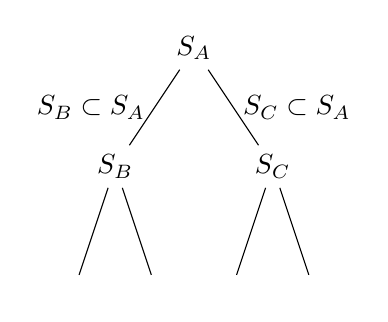
\begin{tikzpicture}
		[level distance=15mm,level/.style={sibling distance=20mm/#1}]
		\node {$S_A$}
		child {node {$S_B$}
				child {node {}}
				child {node {}}
				edge from parent node[left,draw=none] {$S_B\subset S_A$}
			}
		child {node {$S_C$}
				child {node {}}
				child {node {}}
				edge from parent node[right,draw=none] {$S_C\subset S_A$}
			};
	\end{tikzpicture}
	\caption{Trust hierarchies represented as subset-trees define retreat strategies.} \label{fig:subset_tree}
\end{figure}

Fig.~\ref{fig:subset_tree}

`Rebasing' network upon strategic retreat.

Retreat strategy in trust hierarchy where root is level $i=0$. Levels represent set containment, $s_{i+1}\subset s_i$. Retreat to smallest i (i.e largest trusted subset). Assume that $r_{i+1}<r_i$. Inequality could work in either direction??


\subsection{Network democratisation}

* The adoption of network policy changes and node membership is inherently democratic.

* Individual trust counters.

* PoCs signs the adopted constitution.

* \textsc{Propose} policy changes. Accepted upon majority.

%In a competitive market the cost of consensus approximates its production cost.

%A market of freedom and equality.

%While consensus is a tradable commodity with market value, a DCN network is able to operate without 

%During the \textsc{Bid} stage of the protocol, bids presented to the network demand $N_C$ units of work to undergo consensus, 1 unit of work per honest consensus participant. 

%The set of PoCs produced during a round of the protocol collectively reveal the compliance of all network nodes. Nodes contribute 1 unit of work to the network for every consensus they faithfully execute, and consume $N_C$ units of work for every submitted \texttt{statement} subject to consensus.

%During the \textsc{Accept} stage all network nodes are additionally required to agree upon the network's ledger state, where compliant nodes from the previous round have their workload tallies incremented by consensus' they faithfully contributed to and decremented by the the workload consumed by \texttt{statements} they submit for consensus.

%* Upon bidding to participate, nodes promise to faithfully participate in consensus via a deposit. During the \textsc{Accept} stage, this requires nodes' work tallies to be at least as large as their promise. The subsequent ledger state deducts promises from the tallies of non-compliant nodes. To incentivise compliance, the required promise amount must exceed the objective cost of execution.

%This policy enforces neutrality between nodes' contributed and consumed consensus load. While compliance ensures the ledger is monetarily neutral, non-compliance results in the destruction of credits via the associated unreturned deposits, and nodes with insufficient credits from a history of non-compliance are unable make promises for future participation and barred from participation. Here network policy must stipulate buy-in mechanisms for the creation of new consensus credits, for example by settling against external ledgers.

%* Supply side highly competitive. Demand side for access to the network, a floating market entity.

%* Economics based on contribution rather than waste.

%* The network’s economy involves only the direct and simultaneous steady-state exchange of contribution towards consensus — monetarily neutral with no dependence on external currency, driven  only by demand for consensus.

%* New nodes buy into the network by pre-contributing sufficient work to afford future payment for consensus. Accumulated credits by contributing more than is requested additionally acts as a buffer against unintended non-compliance, for example as a result of communications failure. If service distraction prevents participation in consensus the buffer ensures the ability to maintain requests. monetarily neutral.

%* Participation in consensus is a mutual exchange of randomness. The economy of the DCN is driven only by its demand.

%* An open ecosystem driven by mutual exchange, equity and consent.